% -------------------------------------------------------------------
\chapter{O Firmware do microcontrolador ESP8266}\label{apendix:esp8266-fw}
% -------------------------------------------------------------------

O \textit{firmware} do microcontrolador ESP8266 foi desenvolvido na linguagem de programação C/C++ utilizando o \textit{Framework} Arduino. O código foi programado na \acrshort*{ide} PlatformIO para o editor de código Microsoft Visual Studio (VSCode). A versão atual do firmware do ESP8266 possui três funcionalidades principais, que são:

\begin{enumerate}
    \item Prover conexão à Internet a um microcontrolador principal, que atua como "mestre", via uma rede \textit{Wi-Fi}
    \item Envio dos dados coletados pelo microcontrolador "mestre" para o servidor web Renovar mediante \textit{POST} \textit{HTTP}
    \item Obter a data e hora atuais de um servidor \acrshort*{ntp}
\end{enumerate}

A Figura \ref{fig:fw-esp-main-flow} mostra um fluxograma do código programado para o microcontrolador ESP8266. Em primeiro lugar, o programa estabelece uma conexão à Internet através de uma rede \textit{Wi-Fi}. Uma vez estabelecida a conexão, o programa se mantém escutando a conexão serial com o microcontrolador "mestre". Para cada solicitação recebida do "mestre", o ESP8266 executa a operação associada à solicitação e envia seu resultado de volta para o "mestre". As mensagens trocadas entre o ESP8266 e o outro microcontrolador são cadeias de caracteres no formato \acrshort{json}.

Na versão atual do \textit{firmware}, o "mestre" pode realizar dois tipos de solicitações. Pode solicitar o envio de uma requisição para a \acrshort*{api} Renovar na forma de POST HTTP com leituras dos sensores ou pode solicitar a data e hora de um servidor \acrshort*{ntp}.

\begin{figure}[h]
    \centering
    \caption{Fluxograma do firmware programado para o microcontrolador ESP8266}
    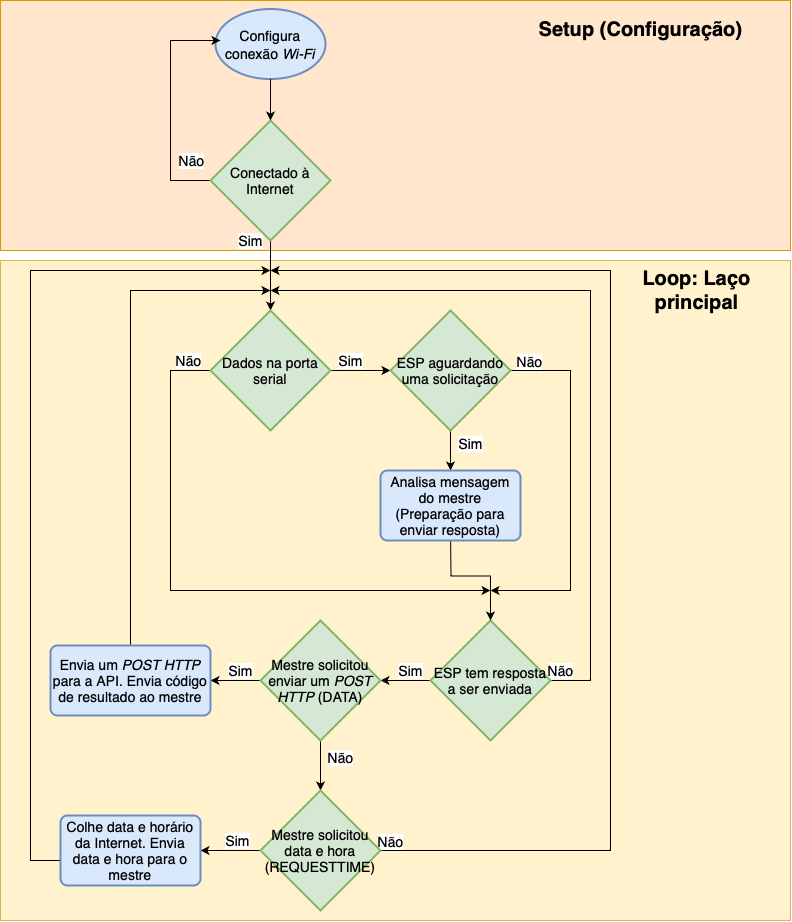
\includegraphics[width=0.5\linewidth]{aftertext//Firmware ESP8266/Figuras/ESP8266 Main flowchart (PT).png}
    \fonte{Desenvolvido pelo autor (2023)}
    \label{fig:fw-esp-main-flow}
\end{figure}

\section{Configuração e conexão \textit{Wi-Fi}}

Conforme mostra o fluxograma da \ref{fig:fw-esp-main-flow}, as primeiras ações que o programa executa são aquelas relacionadas ao estabelecimento da conexão à Internet via rede \textit{Wi-Fi} e a comunicação serial com o microcontrolador "mestre". Isso é realizado na função \texttt{setup()} conforme mostrado no código da Lista \ref{code:esp-setup}.

\begin{lstlisting}[language=C++, caption=Definição dos identificadores dos sensores de um dispositivo]
    void setup() 
    {
        Serial.begin(9600UL);
        Serial.print(F("+STARTESP;"));
        setup_wifi_connection<NUM_WIFIS>(wifiCreds);
        espHTTP.set_available(true);
        espSerial.set_status(WT_REQUEST);
        Serial.print(F("+ESPREADY;"));
    }
\end{lstlisting}
\label{code:esp-setup}

Primeiramente o programa inicializa a porta serial do ESP8266 a uma taxa de transmissão de 9600 bauds e imprime a mensagem \texttt{‘+STARTESP’}, indicando ao mestre que o programa foi inicializado. A função \texttt{setup\_wifi\_connection()} estabelece a conexão em uma rede \textit{Wi-Fi} previamente armazenada na variável \texttt{wifiCreds}. Por fim, uma vez estabelecida a conexão, o objeto \texttt{espSerial} que armazena o estado da comunicação serial é setado para \texttt{WT\_REQUEST} e a mensagem \texttt{'+ESPREADY'} é impressa, indicando que o ESP8266 está aguardando por uma solicitação do microcontrolador "mestre". A partir desse ponto o objeto \texttt{espHTTP} executa as requisições à \acrshort*{api} Renovar através do protocolo \textit{HTTP}. A continuação são descritos os objetos, constantes e funções usados nesta parte do código.

\subsection{\texttt{NUM\_WIFIS}}

Esta constante define a quantidade de redes \textit{Wi-Fi} com as quais o ESP8266 tentará estabelecer uma conexão. Esta constante deve ser declarada antes do objeto \texttt{wifiCreds} e antes de invocar a função \texttt{setup\_wifi\_connection()}.

\subsection{\texttt{WiFiCredentials wifiCreds[]}}

Esta variável é uma lista de objetos do tipo \texttt{WiFiCredentials}. Esta matriz armazena o \acrshort*{ssid} da rede, a senha e o nome de usuário (este último apenas em redes \textit{WPA3 ENTERPRISE}). A lista \texttt{wifiCreds} deve ser declarada antes da função \texttt{setup()}, conforme se mostra no códio da Lista \ref{code:esp-wifi-creds}. O tamanho da lista vai depender do valor da constante \texttt{NUM\_WIFIS}.

\begin{lstlisting}[language=C++, caption=Definição dos identificadores dos sensores de um dispositivo]
    /*Credenciais de uma rede empresarial WPA3*/
    const WiFiCredentials CRED_1("ssid1", "senha1", ENTERPRISE, "nomedeusuario1");

    /*Credenciais das redes pessoais WPA3*/
    const WiFiCredentials CRED_2("ssid2", "senha2", PERSONAL);
    const WiFiCredentials CRED_3("ssid3", "senha3", PERSONAL);

    /*Declara o array wifiCreds*/
    const WiFiCredentials wifiCreds[NUM_WIFIS] = { CRED_1, CRED_2, CRED_3 };
\end{lstlisting}
\label{code:esp-wifi-creds}

\subsection{\texttt{setup\_wifi\_connection<NUM\_WIFIS>(wifiCreds)}}

Esta função estabelece uma conexão a uma rede \textit{Wi-Fi}. É definido como um \textit{template} que recebe a quantidade de redes \textit{Wi-Fi} armazenadas em \texttt{wifiCreds}.

\subsection{\texttt{espHTTP}}

Esta variável é um objeto da classe \texttt{HTTPHandler}, definida no arquivo \texttt{esp-iot.h}, cujo objetivo é encapsular as funcionalidades relacionadas às operações \textit{HTTP}.

\subsection{\texttt{espSerial}}

Esta variável é um objeto da classe \texttt{ESPSerialHandler}, definida no arquivo \texttt{esp-serial-iot.h}. O objetivo deste objeto é encapsular as funcionalidades relacionadas à comunicação serial entre o ESP8266 e o microcontrolador mestre. Dependendo do estado deste objeto, o ESP8266 pode ler uma mensagem serial do mestre, ou executar uma determinada operação e enviar seu resultado de volta ao mestre. Para a versão atual do firmware, foram implementados dois estados:

\texttt{WT\_REQUEST}: Indica que o ESP8266 não recebeu nenhuma solicitação do mestre e está aguardando até receber uma nova.
\texttt{WT\_RESPONSE}: Indica que o ESP8266 recebeu alguma nova solicitação do mestre e está realizando as operações para enviar uma resposta.

\subsection{\texttt{Serial}}

Este é um objeto do framework Arduino para controlar a comunicação serial.

\section{O laço principal}

O laço principal do programa é executado dentro da função \texttt{loop()}, conforme mostrado no código abaixo. Esta função é responsável por monitorar a porta serial do ESP8266 e atender às solicitações do "mestre", conforme já ilustrado na Figura \ref{fig:fw-esp-main-flow}.

\begin{lstlisting}[language=C++, caption=Laço principal do programa]
void loop() 
{
    static CommandTypes _cmdType = ERROR;

    if(Serial.available())
    { 
        String serial_Str = Serial.readStringUntil(';');
        if(espSerial.get_status() == WT_REQUEST)  _cmdType = espSerial.parse(serial_Str);
        Serial.flush();
    }
    if(espSerial.get_status() == WT_RESPONSE)
    {
        espSerial.set_status(WT_REQUEST);
        switch (_cmdType)
        {
            case DATA:
            {
                static uint8_t _numberOfPostTries = 0;
                #define MAX_NUM_TRIES 3
                int code = espHTTP.post(HOST, PORT, URL, espSerial.get_data());
                
                if(code <= 0 && WiFi.status() != WL_CONNECTED)
                {
                    setup_wifi_connection<NUM_WIFIS>(wifiCreds);
                    if(++_numberOfPostTries >= MAX_NUM_TRIES-1) ESP.restart();
                }
                else  espSerial.send_http_code(code, Serial);
                break;
            }

            case REQUESTTIME:
            {
                static uint8_t _numberOfTries = 0;
                #define MAX_NUM_TRIES 3
                time_t t = get_time(TIMEZONE_SEC,DAYLIGTHOFFSET_SEC);
                if(!t && WiFi.status() != WL_CONNECTED)
                {
                    setup_wifi_connection<NUM_WIFIS>(wifiCreds);
                    if(++_numberOfTries >= MAX_NUM_TRIES-1) ESP.restart();
                }
                else  espSerial.send_time(t, Serial);
                break;
            }
            
            default:
            {
                break;
            }
        }
    }
}
\end{lstlisting}
\label{code:esp-loop}

\subsection*{Verificação das solicitações do "mestre"}

Sempre que houver dados na porta serial e o estado da comunicação serial (armazenado no objeto \texttt{espSerial}) for “aguardando solicitação” (\texttt{WT\_REQUEST}), o mesmo objeto \texttt{espSerial} analisará a cadeia de caracteres recebida do "mestre" para determinar o tipo de solicitação que recebeu. Isso é feito dentro do primeiro \texttt{if} da função \texttt{loop()}, conforme mostrado no código da Lista \ref{code:esp-serial-check}.

\begin{lstlisting}[language=C++, caption=Código para verificar as solicitações do mestre]
if(Serial.available())
{ 
    String serial_Str = Serial.readStringUntil(';');
    if(espSerial.get_status() == WT_REQUEST)  _cmdType = espSerial.parse(serial_Str);
    Serial.flush();
}
\end{lstlisting}
\label{code:esp-serial-check}

Uma vez analisada a mensagem do "mestre", \texttt{espSerial} definirá seu estado para “aguardando resposta” (\texttt{WT\_RESPONSE}), indicando que uma operação está em execução e uma resposta deve ser enviada de volta para o mestre (isso é feito internamente no a função parse). Se o status de \texttt{espSerial} for \texttt{WT\_RESPONSE}, o programa realizará uma operação \texttt{switch} para determinar qual operação o microcontrolador deve executar a seguir (fluxograma da Figura \ref{fig:fw-esp-main-flow}). A seleção da operação dependerá do tipo de solicitação enviado pelo mestre. O tipo de solicitação é armazenado na variável \texttt{\_cmdType} como resultado da operação \texttt{parse()} executada por \texttt{espSerial}. A Figura \ref{fig:fw-esp-comm-att} mostra esse processo.

\begin{figure}[h]
    \centering
    \caption{Processo de atendimento a uma solicitação do mestre}
    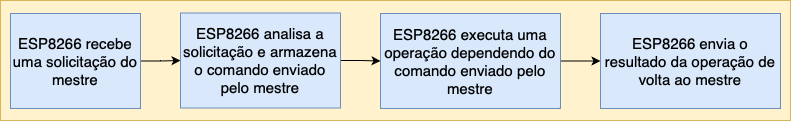
\includegraphics[width=0.9\linewidth]{aftertext//Firmware ESP8266/Figuras/ESP8266 sequence of comm operations (PT).png}
    \fonte{Desenvolvido pelo autor (2023)}
    \label{fig:fw-esp-comm-att}
\end{figure}

Na versão atual do firmware, o ESP8266 aceita dois tipos de solicitações ou comandos do mestre: (1) uma solicitação para enviar uma requisição à \acrshort*{api} Renovar via um \textit{POST HTTP} ou (2) uma solicitação de data e horário. A estrutura de uma mensagem de solicitação é mostrada no \acrshort{json} da Lista \ref{code:esp-wifi-json}. Depois que o objeto \texttt{espSerial} processa a mensagem do mestre, ele armazena o tipo de solicitação na variável \texttt{\_cmdType}. Esta variável é uma enumeração do tipo \texttt{CommandTypes} e, para a versão atual, pode conter os valores \texttt{ERROR}, \texttt{DATA} e \texttt{REQUESTTIME}, veja a Tabela \ref{tab:fw-esp-commands}.

\begin{lstlisting}[language=C++, caption=O formato da string JSON trocada entre o ESP8266 e o mestre]
{
    'type': // The type of the request. Could be 1 (DATA) or 2 (REQUESTTIME)
    'body': // The body of the request. Only used when the master is sending data (DATA)
}
\end{lstlisting}
\label{code:esp-wifi-json}

\begin{table}[h]
    \centering
    \caption{Tipos de solicitações representadas no tipo \texttt{CommandTypes}}
    \label{tab:fw-esp-commands}
    \begin{tabularx}{0.98\textwidth}[h]{
         >{\raggedright\hsize=.32\hsize\arraybackslash}X
         >{\raggedright\hsize=.12\hsize\arraybackslash}X 
         >{\raggedright\arraybackslash}X
         >{\raggedleft\hsize=.55\hsize\arraybackslash}X }
         \hline
         \texttt{CommandTypes} & \textbf{Valor}  & \textbf{Descrição} & \textbf{Resposta do mestre} \\
         \hline
         \texttt{ERROR} & 0 & Este comando indica que ocorreu um erro na comunicação do mestre com o ESP8266. Normalmente usado do ESP8266 para o mestre & É a resposta em caso de erro de comunicação \\
        \hline
        \texttt{DATA} & 1 & Este comando indica que o mestre enviou os dados para uma postagem HTTP e está aguardando o código HTTP retornado do servidor Web como resposta à postagem & O código HTTP retornado pelo servidor Web após a postagem \\
        \hline
        \texttt{REQUESTTIME} & 2 & Este comando indica que o mestre está solicitando a hora de um servidor NTP & O carimbo de data/hora obtido pelo servidor NTP \\
        \hline
    \end{tabularx}
    \fonte{Desenvolvido pelo autor (2023)}
\end{table}

\subsection{O comando \texttt{DATA}: enviando um \texttt{POST HTTP} para a API Renovar}

O código executado quando o "mestre" solicita o envio de um \textit{POST HTTP} é mostrado na Lista \ref*{code:esp-wifi-data-sequence}. O objeto \texttt{espHTTP} faz uma requisição tipo \textit{POST} para a \acrshort{api} hospedada em um servidor web identificado por um \textit{HOST} (hospedeiro), uma Porta e uma \acrshort{url} específica. Os dados enviados no \textit{POST} são os mesmos enviados anteriormente pelo mestre. Estes dados são acessados pelo método \texttt{get\_data()} de \texttt{espSerial}. O código retornado dessa operação é enviado como resposta ao "mestre" para manter controle das suas operações. Caso o código for de falha e o ESP8266 não estiver conectado à rede \textit{Wi-Fi}, o programa tentará se reconectar à rede e repassar os dados no máximo por três tentativas. Se, por outro lado, o código for de falha mas o ESP8266 estiver conectado a uma rede \textit{Wi-Fi}, o programa tentará enviar a mesma requisição indefinidamente até que o mestre envie uma nova solicitação. A Figura \ref*{fig:fw-esp-data-sequence} apresenta um fluxograma que representa esse processo. 

\begin{figure}[h]
    \centering
    \caption{Fluxograma do processo após uma solicitação de DATA do mestre.}
    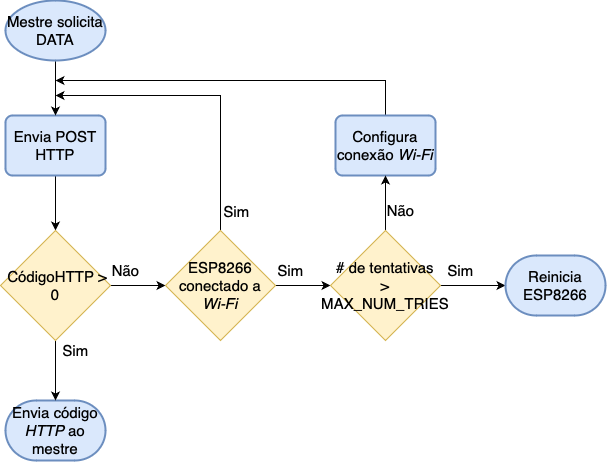
\includegraphics[width=0.75\linewidth]{aftertext//Firmware ESP8266/Figuras/ESP8266 DATA sequence (PT).png}
    \fonte{Desenvolvido pelo autor (2023)}
    \label{fig:fw-esp-data-sequence}
\end{figure}

\begin{lstlisting}[language=C++, caption=Sequencia de operações no comando DATA]
case DATA:
{
  static uint8_t _numberOfPostTries = 0;
  #define MAX_NUM_TRIES 3
  int code = espHTTP.post(HOST, PORT, URL, espSerial.get_data());
        
  if(code <= 0 && WiFi.status() != WL_CONNECTED)
  {
    setup_wifi_connection<NUM_WIFIS>(wifiCreds);
    if(++_numberOfPostTries >= MAX_NUM_TRIES-1) ESP.restart();
  }
  else  espSerial.send_http_code(code, Serial);
  break;
}
\end{lstlisting}
\label{code:esp-wifi-data-sequence}

Os valores de \texttt{HOST}, \texttt{PORT} e \texttt{URL} são definidos no arquivo \texttt{iot-generic.h} conforme se mostra abaixo; eles representam o \textit{endpoint} para enviar requisições à \acrshort*{api} Renovar.

\begin{lstlisting}[language=C++]
#define HOST  F("renovar.lcqar.ufsc.br")
#define PORT  8080UL
#define URL   F("/sample/")
\end{lstlisting}

\subsection*{O comando \texttt{REQUESTTIME}: obtendo a hora de um servidor \acrshort*{ntp}}

O código executado quando o ESP8266 recebe uma solicitação de horário é mostrado na Lista \ref*{code:esp-wifi-time-sequence}. A função \texttt{get\_time()} é definida no arquivo \texttt{esp-iot.h} para obter a data e hora atuais desde um servidor 
\acrshort{ntp}. O valor retornado dessa operação é enviado como resposta ao "mestre". Caso o valor for zero e o ESP8266 não esteja conectado à rede \texttt{Wi-Fi}, o programa tentará se reconectar à rede e obter o horário da Internet por no máximo três tentativas. Por outro lado, se o valor for zero, mas o ESP8266 estiver conectado a uma rede Wi-Fi, o programa tentará obter o horário da Internet indefinidamente até receber uma nova solicitação. A Figura \ref*{fig:fw-esp-time-sequence} apresenta um fluxograma que representa esse processo.

\begin{figure}[h]
    \centering
    \caption{Fluxograma do processo após uma solicitação TIME do mestre}
    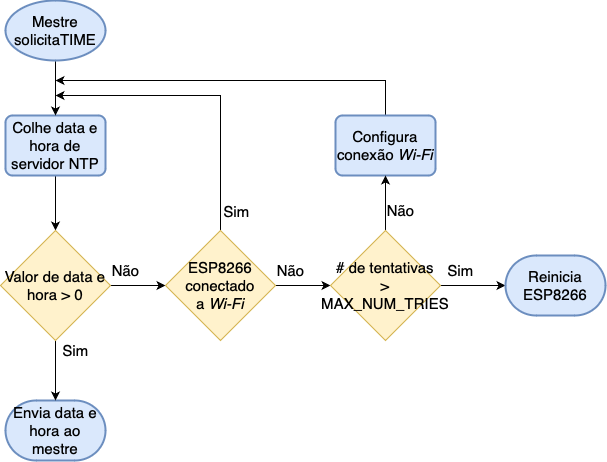
\includegraphics[width=0.75\linewidth]{aftertext//Firmware ESP8266/Figuras/ESP8266 TIME sequence(PT).png}
    \fonte{Desenvolvido pelo autor (2023)}
    \label{fig:fw-esp-time-sequence}
\end{figure}

\begin{lstlisting}[language=C++, caption=Sequencia de operações no comando REQUESTTIME]
case REQUESTTIME:
{
  static uint8_t _numberOfTries = 0;
  #define MAX_NUM_TRIES 3
  time_t t = get_time(TIMEZONE_SEC,DAYLIGTHOFFSET_SEC);
  if(!t && WiFi.status() != WL_CONNECTED)
  {
    setup_wifi_connection<NUM_WIFIS>(wifiCreds);
    if(++_numberOfTries >= MAX_NUM_TRIES-1) ESP.restart();
  }
  else  espSerial.send_time(t, Serial);
  break;
}
\end{lstlisting}
\label{code:esp-wifi-time-sequence}

A função \texttt{get\_time()} recebe os parâmetros \texttt{TIMEZONE\_SEC} e \texttt{DAYLIGTHOFFSET\_SEC}, definidos anteriormente no arquivo \texttt{main.cpp}. O exemplo abaixo mostra como definir esses dois parâmetros para a aplicação no Brasil. \texttt{TIMEZONE\_SEC} é o fuso horário onde o monitor será instalado, convertido a segundos. \texttt{DAYLIGTHOFFSET\_SEC} define o deslocamento, em segundos, para o horário de verão, nesse caso foi definido como zero.

\begin{lstlisting}[language=C++]
#define TIMEZONE_SEC        -3*3600
#define DAYLIGTHOFFSET_SEC  0*3600
\end{lstlisting}